\begin{sectionheader}{Section II}
    \textbf{80 marks\\
    Attempt Questions 21--34\\
    Allow about 2 hours 25 minutes for this section}
    
    Answer the questions in the spaces provided. These spaces provide\\ guidance for the expected length of response.
    
    Show all relevant working in questions involving calculations.

    No extra writing space for you verbose nerds.
\end{sectionheader}

\begin{shortanswer}         % short answer section

%#############################################################################################################%
%################################# QUESTION 21 ##########################################################%
%#############################################################################################################%
\begin{shortquestion}{6} % start booklet question

A car is driving in uniform circular motion on an inclined plane as depicted below.
\begin{center}
    

\tikzset{every picture/.style={line width=0.75pt}} %set default line width to 0.75pt        

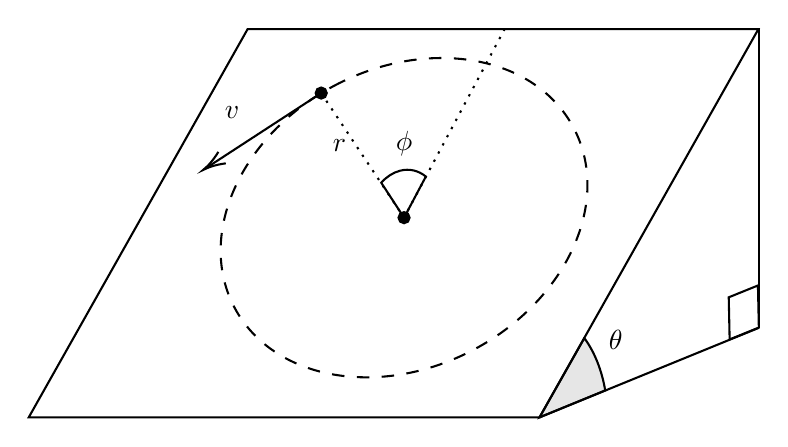
\begin{tikzpicture}[x=0.75pt,y=0.75pt,yscale=-1,xscale=1]
%uncomment if require: \path (0,300); %set diagram left start at 0, and has height of 300

%Straight Lines [id:da47922463191494025] 
\draw    (404.77,80.73) -- (404.77,224.73) ;
%Shape: Pie [id:dp6052033696960859] 
\draw  [color={rgb, 255:red, 0; green, 0; blue, 0 }  ,draw opacity=1 ][fill={rgb, 255:red, 216; green, 216; blue, 216 }  ,fill opacity=0.64 ] (320.7,229.78) .. controls (325.52,236.35) and (329.08,245.08) .. (330.76,255.01) -- (299.09,268) -- cycle ;
%Shape: Parallelogram [id:dp3636291479456979] 
\draw   (158.47,80.92) -- (404.56,80.92) -- (299.09,268) -- (53,268) -- cycle ;
%Straight Lines [id:da07860560767008584] 
\draw    (404.56,224.92) -- (299.09,268) ;
%Shape: Ellipse [id:dp33809398213922104] 
\draw  [dash pattern={on 4.5pt off 4.5pt}] (200.07,108.27) .. controls (245.16,84.3) and (296.83,93.29) .. (315.47,128.36) .. controls (334.12,163.43) and (312.68,211.29) .. (267.6,235.26) .. controls (222.51,259.24) and (170.84,250.24) .. (152.2,215.18) .. controls (133.55,180.11) and (154.99,132.25) .. (200.07,108.27) -- cycle ;
%Shape: Circle [id:dp9660949777850081] 
\draw  [fill={rgb, 255:red, 0; green, 0; blue, 0 }  ,fill opacity=1 ] (191.25,111.74) .. controls (191.25,110.26) and (192.45,109.06) .. (193.92,109.06) .. controls (195.4,109.06) and (196.6,110.26) .. (196.6,111.74) .. controls (196.6,113.21) and (195.4,114.41) .. (193.92,114.41) .. controls (192.45,114.41) and (191.25,113.21) .. (191.25,111.74) -- cycle ;
%Straight Lines [id:da054710075011608295] 
\draw    (193.92,111.74) -- (138.68,147.71) ;
\draw [shift={(137,148.8)}, rotate = 326.93] [color={rgb, 255:red, 0; green, 0; blue, 0 }  ][line width=0.75]    (10.93,-3.29) .. controls (6.95,-1.4) and (3.31,-0.3) .. (0,0) .. controls (3.31,0.3) and (6.95,1.4) .. (10.93,3.29)   ;
%Shape: Circle [id:dp16939027997095324] 
\draw  [fill={rgb, 255:red, 0; green, 0; blue, 0 }  ,fill opacity=1 ] (231.16,171.77) .. controls (231.16,170.29) and (232.36,169.09) .. (233.84,169.09) .. controls (235.31,169.09) and (236.51,170.29) .. (236.51,171.77) .. controls (236.51,173.25) and (235.31,174.44) .. (233.84,174.44) .. controls (232.36,174.44) and (231.16,173.25) .. (231.16,171.77) -- cycle ;
%Straight Lines [id:da20455724854353496] 
\draw  [dash pattern={on 0.84pt off 2.51pt}]  (193.92,111.74) -- (233.84,171.77) ;
%Shape: Parallelogram [id:dp8445337594196616] 
\draw   (404.77,224.73) -- (404.34,204.44) -- (390.27,210.14) -- (390.7,230.43) -- cycle ;
%Straight Lines [id:da05309378649652152] 
\draw  [dash pattern={on 0.84pt off 2.51pt}]  (282.35,80.77) -- (233.84,171.77) ;
%Shape: Pie [id:dp8762145687246736] 
\draw  [color={rgb, 255:red, 0; green, 0; blue, 0 }  ,draw opacity=1 ] (222.85,154.93) .. controls (225.38,152.09) and (228.47,150.03) .. (231.89,149.15) .. controls (236.49,147.96) and (240.87,149.11) .. (244.34,151.96) -- (233.84,171.77) -- cycle ;

% Text Node
\draw (331,224.4) node [anchor=north west][inner sep=0.75pt]    {$\theta $};
% Text Node
\draw (198,132.8) node [anchor=north west][inner sep=0.75pt]    {$r$};
% Text Node
\draw (146,116.6) node [anchor=north west][inner sep=0.75pt]    {$v$};
% Text Node
\draw (228.4,128.8) node [anchor=north west][inner sep=0.75pt]    {$\phi $};


\end{tikzpicture}   
\end{center}
    
The angle of inclination $\theta = 30^{\circ}$. The radius is $r = 5\,\si{\meter}$. The velocity of the car is $v = 3\,\si{\meter\per\second}$.
The mass of the car is $m = 1000\,\si{\kg}$.

\begin{enumerate}           % start question parts
    \item\mrks{2} Calculate the component of weight force acting parallel to the ramp.
    \lines{5}
    \questionbreak
    \item\mrks{4} Hence calculate the magnitude of friction force when $\phi = 45^{\circ}$.
    \lines{10}

    \item\mrks{3} Calculate the work done by friction on the car between $\phi = 0$ and $\phi = 180^{\circ}$.
    \lines{8}
    
    \questionend                % End of question...
\end{enumerate}                 % end question parts
\end{shortquestion}           % end booklet question

\pagebreak

%#############################################################################################################%
%################################# QUESTION 22 ##########################################################%
%#############################################################################################################%
\begin{shortquestion}{4}        % start short question

An AC generator produces a voltage

\begin{center}
    

\tikzset{every picture/.style={line width=0.75pt}} %set default line width to 0.75pt        

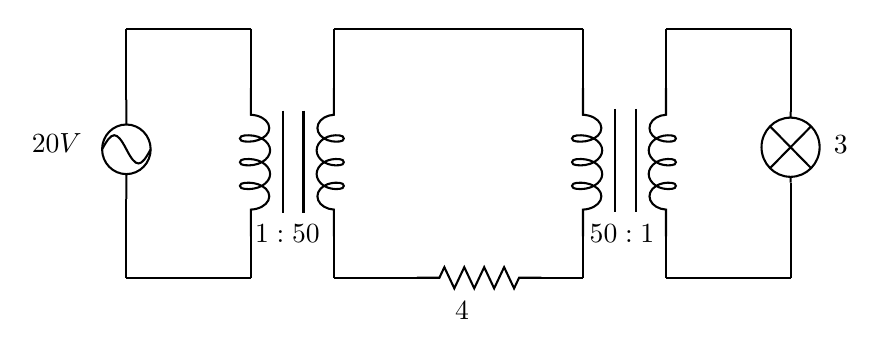
\begin{tikzpicture}[x=0.75pt,y=0.75pt,yscale=-1,xscale=1]
%uncomment if require: \path (0,300); %set diagram left start at 0, and has height of 300

%Shape: Inductor (Air Core) [id:dp5461500128640597] 
\draw   (194.65,105.82) -- (194.65,118.67) .. controls (198.56,118.85) and (201.91,120.63) .. (203.07,123.16) .. controls (204.24,125.68) and (203,128.43) .. (199.94,130.09) .. controls (197.56,131.36) and (194.47,131.88) .. (191.48,131.52) .. controls (190.31,131.52) and (189.36,130.88) .. (189.36,130.09) .. controls (189.36,129.3) and (190.31,128.66) .. (191.48,128.66) .. controls (194.47,128.29) and (197.56,128.81) .. (199.94,130.09) .. controls (202.48,131.57) and (203.92,133.64) .. (203.92,135.8) .. controls (203.92,137.96) and (202.48,140.03) .. (199.94,141.51) .. controls (197.56,142.79) and (194.47,143.31) .. (191.48,142.94) .. controls (190.31,142.94) and (189.36,142.3) .. (189.36,141.51) .. controls (189.36,140.72) and (190.31,140.08) .. (191.48,140.08) .. controls (194.47,139.72) and (197.56,140.24) .. (199.94,141.51) .. controls (202.48,143) and (203.92,145.06) .. (203.92,147.22) .. controls (203.92,149.38) and (202.48,151.45) .. (199.94,152.93) .. controls (197.56,154.21) and (194.47,154.73) .. (191.48,154.36) .. controls (190.31,154.36) and (189.36,153.72) .. (189.36,152.93) .. controls (189.36,152.15) and (190.31,151.51) .. (191.48,151.51) .. controls (194.47,151.14) and (197.56,151.66) .. (199.94,152.93) .. controls (203,154.59) and (204.24,157.34) .. (203.07,159.86) .. controls (201.91,162.39) and (198.56,164.17) .. (194.65,164.36) -- (194.65,177.21) ;
%Straight Lines [id:da9952902044984588] 
\draw    (134.65,77.21) -- (134.65,111.42) ;
%Straight Lines [id:da3652897250844733] 
\draw    (134.65,159.21) -- (134.65,197.21) ;
%Straight Lines [id:da4589520493076342] 
\draw    (134.65,77.21) -- (194.65,77.21) ;
%Straight Lines [id:da6403365683726014] 
\draw    (134.65,197.21) -- (194.65,197.21) ;
%Straight Lines [id:da01246549017342824] 
\draw    (194.65,197.21) -- (194.65,177.21) ;
%Straight Lines [id:da3125921503790394] 
\draw    (194.65,77.21) -- (194.65,105.82) ;
%Shape: Inductor (Air Core) [id:dp5406179172495555] 
\draw   (234.65,105.82) -- (234.65,118.67) .. controls (231.14,118.85) and (228.13,120.63) .. (227.08,123.16) .. controls (226.03,125.68) and (227.14,128.43) .. (229.9,130.09) .. controls (232.04,131.36) and (234.81,131.88) .. (237.51,131.52) .. controls (238.56,131.52) and (239.41,130.88) .. (239.41,130.09) .. controls (239.41,129.3) and (238.56,128.66) .. (237.51,128.66) .. controls (234.81,128.29) and (232.04,128.81) .. (229.9,130.09) .. controls (227.61,131.57) and (226.31,133.64) .. (226.31,135.8) .. controls (226.31,137.96) and (227.61,140.03) .. (229.9,141.51) .. controls (232.04,142.79) and (234.81,143.31) .. (237.51,142.94) .. controls (238.56,142.94) and (239.41,142.3) .. (239.41,141.51) .. controls (239.41,140.72) and (238.56,140.08) .. (237.51,140.08) .. controls (234.81,139.72) and (232.04,140.24) .. (229.9,141.51) .. controls (227.61,143) and (226.31,145.06) .. (226.31,147.22) .. controls (226.31,149.38) and (227.61,151.45) .. (229.9,152.93) .. controls (232.04,154.21) and (234.81,154.73) .. (237.51,154.36) .. controls (238.56,154.36) and (239.41,153.72) .. (239.41,152.93) .. controls (239.41,152.15) and (238.56,151.51) .. (237.51,151.51) .. controls (234.81,151.14) and (232.04,151.66) .. (229.9,152.93) .. controls (227.14,154.59) and (226.03,157.34) .. (227.08,159.86) .. controls (228.13,162.39) and (231.14,164.17) .. (234.65,164.36) -- (234.65,177.21) ;
%Straight Lines [id:da13232805081676102] 
\draw    (209.98,116.62) -- (209.98,166.22) ;
%Straight Lines [id:da8335900506026364] 
\draw    (219.98,116.62) -- (219.98,166.22) ;
%Straight Lines [id:da5325963938688358] 
\draw    (234.65,177.21) -- (234.65,197.21) ;
%Straight Lines [id:da3480107769549703] 
\draw    (234.65,77.21) -- (234.65,105.82) ;
%Straight Lines [id:da512117268831449] 
\draw    (234.65,77.21) -- (354.65,77.21) ;
%Straight Lines [id:da775573162249596] 
\draw    (234.65,197.21) -- (274.65,197.21) ;
%Straight Lines [id:da009036849539182157] 
\draw    (354.65,197.21) -- (334.65,197.21) ;
%Shape: Resistor [id:dp05350028975024035] 
\draw   (274.65,197.21) -- (285.45,197.21) -- (287.85,192.11) -- (292.65,202.3) -- (297.45,192.11) -- (302.25,202.3) -- (307.05,192.11) -- (311.85,202.3) -- (316.65,192.11) -- (321.45,202.3) -- (323.85,197.21) -- (334.65,197.21) ;
%Straight Lines [id:da6339477963374349] 
\draw    (354.65,177.21) -- (354.65,197.21) ;
%Straight Lines [id:da36489068599925467] 
\draw    (354.65,77.21) -- (354.65,105.82) ;
%Shape: Inductor (Air Core) [id:dp1285512322094755] 
\draw   (354.65,105.82) -- (354.65,118.67) .. controls (358.56,118.85) and (361.91,120.63) .. (363.07,123.16) .. controls (364.24,125.68) and (363,128.43) .. (359.94,130.09) .. controls (357.56,131.36) and (354.47,131.88) .. (351.48,131.52) .. controls (350.31,131.52) and (349.36,130.88) .. (349.36,130.09) .. controls (349.36,129.3) and (350.31,128.66) .. (351.48,128.66) .. controls (354.47,128.29) and (357.56,128.81) .. (359.94,130.09) .. controls (362.48,131.57) and (363.92,133.64) .. (363.92,135.8) .. controls (363.92,137.96) and (362.48,140.03) .. (359.94,141.51) .. controls (357.56,142.79) and (354.47,143.31) .. (351.48,142.94) .. controls (350.31,142.94) and (349.36,142.3) .. (349.36,141.51) .. controls (349.36,140.72) and (350.31,140.08) .. (351.48,140.08) .. controls (354.47,139.72) and (357.56,140.24) .. (359.94,141.51) .. controls (362.48,143) and (363.92,145.06) .. (363.92,147.22) .. controls (363.92,149.38) and (362.48,151.45) .. (359.94,152.93) .. controls (357.56,154.21) and (354.47,154.73) .. (351.48,154.36) .. controls (350.31,154.36) and (349.36,153.72) .. (349.36,152.93) .. controls (349.36,152.15) and (350.31,151.51) .. (351.48,151.51) .. controls (354.47,151.14) and (357.56,151.66) .. (359.94,152.93) .. controls (363,154.59) and (364.24,157.34) .. (363.07,159.86) .. controls (361.91,162.39) and (358.56,164.17) .. (354.65,164.36) -- (354.65,177.21) ;
%Shape: Output [id:dp5861176659665983] 
\draw   (134.65,147.26) .. controls (128.2,147.26) and (122.96,141.91) .. (122.96,135.31) .. controls (122.96,128.71) and (128.2,123.36) .. (134.65,123.36) .. controls (141.11,123.36) and (146.35,128.71) .. (146.35,135.31) .. controls (146.35,141.91) and (141.11,147.26) .. (134.65,147.26) -- cycle (134.65,159.21) -- (134.65,147.26) (134.65,111.42) -- (134.65,123.36) ;
%Shape: Sine Wave Form [id:dp7857874556537092] 
\draw   (122.96,135.31) .. controls (127.72,126.3) and (129.96,126.25) .. (134.65,135.31) .. controls (139.34,144.37) and (141.54,144.43) .. (146.35,135.31) ;
%Shape: Inductor (Air Core) [id:dp9236526554549926] 
\draw   (394.65,105.82) -- (394.65,118.67) .. controls (391.14,118.85) and (388.13,120.63) .. (387.08,123.16) .. controls (386.03,125.68) and (387.14,128.43) .. (389.9,130.09) .. controls (392.04,131.36) and (394.81,131.88) .. (397.51,131.52) .. controls (398.56,131.52) and (399.41,130.88) .. (399.41,130.09) .. controls (399.41,129.3) and (398.56,128.66) .. (397.51,128.66) .. controls (394.81,128.29) and (392.04,128.81) .. (389.9,130.09) .. controls (387.61,131.57) and (386.31,133.64) .. (386.31,135.8) .. controls (386.31,137.96) and (387.61,140.03) .. (389.9,141.51) .. controls (392.04,142.79) and (394.81,143.31) .. (397.51,142.94) .. controls (398.56,142.94) and (399.41,142.3) .. (399.41,141.51) .. controls (399.41,140.72) and (398.56,140.08) .. (397.51,140.08) .. controls (394.81,139.72) and (392.04,140.24) .. (389.9,141.51) .. controls (387.61,143) and (386.31,145.06) .. (386.31,147.22) .. controls (386.31,149.38) and (387.61,151.45) .. (389.9,152.93) .. controls (392.04,154.21) and (394.81,154.73) .. (397.51,154.36) .. controls (398.56,154.36) and (399.41,153.72) .. (399.41,152.93) .. controls (399.41,152.15) and (398.56,151.51) .. (397.51,151.51) .. controls (394.81,151.14) and (392.04,151.66) .. (389.9,152.93) .. controls (387.14,154.59) and (386.03,157.34) .. (387.08,159.86) .. controls (388.13,162.39) and (391.14,164.17) .. (394.65,164.36) -- (394.65,177.21) ;
%Straight Lines [id:da2969527901076576] 
\draw    (394.65,177.21) -- (394.65,197.21) ;
%Straight Lines [id:da36335635066850225] 
\draw    (394.65,77.21) -- (394.65,105.82) ;
%Straight Lines [id:da2218004659627022] 
\draw    (394.65,77.21) -- (454.65,77.21) ;
%Straight Lines [id:da764479476245228] 
\draw    (394.65,197.21) -- (454.65,197.21) ;
%Shape: Light Bulb [id:dp45962964564088793] 
\draw   (454.65,120.06) .. controls (462.38,120.06) and (468.65,126.44) .. (468.65,134.31) .. controls (468.65,142.18) and (462.38,148.57) .. (454.65,148.57) .. controls (446.92,148.57) and (440.66,142.18) .. (440.66,134.31) .. controls (440.66,126.44) and (446.92,120.06) .. (454.65,120.06) -- cycle (464.62,124.16) -- (444.69,144.46) (464.62,144.46) -- (444.69,124.16) (454.65,117.21) -- (454.65,120.06) (454.65,148.57) -- (454.65,151.42) ;
%Straight Lines [id:da5341965556100576] 
\draw    (454.65,77.21) -- (454.65,117.21) ;
%Straight Lines [id:da8479052301350332] 
\draw    (454.65,151.42) -- (454.65,197.21) ;
%Straight Lines [id:da17854229708027547] 
\draw    (369.98,115.82) -- (369.98,165.42) ;
%Straight Lines [id:da44385604546880586] 
\draw    (379.98,115.82) -- (379.98,165.42) ;

% Text Node
\draw (87.6,126.2) node [anchor=north west][inner sep=0.75pt]    {$20V$};
% Text Node
\draw (291.6,207.4) node [anchor=north west][inner sep=0.75pt]    {$4\si{\ohm}$};
% Text Node
\draw (474,127.4) node [anchor=north west][inner sep=0.75pt]    {$3\si{\ohm}$};
% Text Node
\draw (195.2,170.2) node [anchor=north west][inner sep=0.75pt]    {$1:50$};
% Text Node
\draw (356.4,170.2) node [anchor=north west][inner sep=0.75pt]    {$50:1$};


\end{tikzpicture}

\end{center}

\begin{enumerate}
    \item\mrks{2} What's nine plus ten.
    \lines{4}
    \item\mrks{2} You stupid.
    \lines{4}
    \questionend
\end{enumerate}

\end{shortquestion}
\pagebreak

%#############################################################################################################%
%################################# QUESTION 23 ##########################################################%
%#############################################################################################################%
\begin{shortquestion}{4}        % start short question
HIHIHIHIHIHI
\pic{images/triangle.png}{7cm}
\begin{enumerate}
    \item\mrks{2} Find the value of $\theta$, correct to the nearest degree.
    \lines{4}
    \item\mrks{2} Find the value of $x$, correct to one decimal place.
    \lines{4}
\end{enumerate}

\end{shortquestion}             % end short question

%#############################################################################################################%
%################################# END OF THE PAPER ##########################################################%
%#############################################################################################################%
\centerbold{End of paper}
\end{shortanswer}               % end short answer section